\input{preamble}

\begin{document}
  \vspace*{0.2in}
  \begin{flushleft}
    % Title must be 250 characters or less.
{\Large
% Please use "sentence case" for title and headings (capitalize only the first word in a title
\textbf\newline{Title of submission to PLOS journals}
}
\newline

    % Insert author names, affiliations and corresponding author email (do not include titles, positions, or degrees).
\\
Name1 Surname\textsuperscript{1,2\Yinyang},
Name2 Surname\textsuperscript{2\Yinyang},
Name3 Surname\textsuperscript{2,3\textcurrency},
Name4 Surname\textsuperscript{2},
Name5 Surname\textsuperscript{2\ddag},
Name6 Surname\textsuperscript{2\ddag},
Name7 Surname\textsuperscript{1,2,3*},
with the Lorem Ipsum Consortium\textsuperscript{\textpilcrow}
\\
\bigskip
\textbf{1} Affiliation Dept/Program/Center, Institution Name, City, State, Country
\\
\textbf{2} Affiliation Dept/Program/Center, Institution Name, City, State, Country
\\
\textbf{3} Affiliation Dept/Program/Center, Institution Name, City, State, Country
\\
\bigskip

% Insert additional author notes using the symbols described below. Insert symbol callouts after author names as necessary.
%
% Remove or comment out the author notes below if they aren't used.
%
% Primary Equal Contribution Note
\Yinyang These authors contributed equally to this work.

% Additional Equal Contribution Note
% Also use this double-dagger symbol for special authorship notes, such as senior authorship.
\ddag These authors also contributed equally to this work.

% Current address notes
\textcurrency Current Address: Dept/Program/Center, Institution Name, City, State, Country % change symbol to "\textcurrency a" if more than one current address note
% \textcurrency b Insert second current address
% \textcurrency c Insert third current address

% Deceased author note
\dag Deceased

% Group/Consortium Author Note
\textpilcrow Membership list can be found in the Acknowledgments section.

% Use the asterisk to denote corresponding authorship and provide email address in note below.
* correspondingauthor@institute.edu

  \end{flushleft}
  \input{head/abstract}

  \linenumbers

  % Use "Eq" instead of "Equation" for equation citations.
\section*{Introduction}
Lorem ipsum dolor sit~\cite{bib1} amet, consectetur adipiscing elit. Curabitur eget porta erat. Morbi consectetur est vel gravida pretium. Suspendisse ut dui eu ante cursus gravida non sed sem. Nullam Eq~(\ref{eq:schemeP}) sapien tellus, commodo id velit id, eleifend volutpat quam. Phasellus mauris velit, dapibus finibus elementum vel, pulvinar non tellus. Nunc pellentesque pretium diam, quis maximus dolor faucibus id.~\cite{bib2} Nunc convallis sodales ante, ut ullamcorper est egestas vitae. Nam sit amet enim ultrices, ultrices elit pulvinar, volutpat risus.

\begin{eqnarray}
\label{eq:schemeP}
	\mathrm{P_Y} = \underbrace{H(Y_n) - H(Y_n|\mathbf{V}^{Y}_{n})}_{S_Y} + \underbrace{H(Y_n|\mathbf{V}^{Y}_{n})- H(Y_n|\mathbf{V}^{X,Y}_{n})}_{T_{X\rightarrow Y}},
\end{eqnarray}

  \section*{Materials and methods}
\subsection*{Etiam eget sapien nibh}

% For figure citations, please use "Fig" instead of "Figure".
% Nulla mi mi, Fig~\ref{fig1} venenatis sed ipsum varius, volutpat euismod diam.
Proin rutrum vel massa non gravida. Quisque tempor sem et dignissim rutrum. Lorem ipsum dolor sit amet, consectetur adipiscing elit. Morbi at justo vitae nulla elementum commodo eu id massa. In vitae diam ac augue semper tincidunt eu ut eros. Fusce fringilla erat porttitor lectus cursus, \nameref{S1_Video} vel sagittis arcu lobortis. Aliquam in enim semper, aliquam massa id, cursus neque. Praesent faucibus semper libero.

% Place figure captions after the first paragraph in which they are cited.
% \begin{figure}[!h]
% \caption{{\bf Bold the figure title.}
% Figure caption text here, please use this space for the figure panel descriptions instead of using subfigure commands. A: Lorem ipsum dolor sit amet. B: Consectetur adipiscing elit.}
% \label{fig1}
% \end{figure}

  % Results and Discussion can be combined.
\section*{Results}
Nulla mi mi, venenatis sed ipsum varius, Table~\ref{table1} volutpat euismod diam. Proin rutrum vel massa non gravida. Quisque tempor sem et dignissim rutrum. Lorem ipsum dolor sit amet, consectetur adipiscing elit. Morbi at justo vitae nulla elementum commodo eu id massa. In vitae diam ac augue semper tincidunt eu ut eros. Fusce fringilla erat porttitor lectus cursus, vel sagittis arcu lobortis. Aliquam in enim semper, aliquam massa id, cursus neque. Praesent faucibus semper libero.

% Place tables after the first paragraph in which they are cited.
\begin{table}[!ht]
\begin{adjustwidth}{-2.25in}{0in} % Comment out/remove adjustwidth environment if table fits in text column.
\centering
\caption{
{\bf Table caption Nulla mi mi, venenatis sed ipsum varius, volutpat euismod diam.}}
\begin{tabular}{|l+l|l|l|l|l|l|l|}
\hline
\multicolumn{4}{|l|}{\bf Heading1} & \multicolumn{4}{|l|}{\bf Heading2}\\ \thickhline
$cell1 row1$ & cell2 row 1 & cell3 row 1 & cell4 row 1 & cell5 row 1 & cell6 row 1 & cell7 row 1 & cell8 row 1\\ \hline
$cell1 row2$ & cell2 row 2 & cell3 row 2 & cell4 row 2 & cell5 row 2 & cell6 row 2 & cell7 row 2 & cell8 row 2\\ \hline
$cell1 row3$ & cell2 row 3 & cell3 row 3 & cell4 row 3 & cell5 row 3 & cell6 row 3 & cell7 row 3 & cell8 row 3\\ \hline
\end{tabular}
\begin{flushleft} Table notes Phasellus venenatis, tortor nec vestibulum mattis, massa tortor interdum felis, nec pellentesque metus tortor nec nisl. Ut ornare mauris tellus, vel dapibus arcu suscipit sed.
\end{flushleft}
\label{table1}
\end{adjustwidth}
\end{table}


%PLOS does not support heading levels beyond the 3rd (no 4th level headings).
\subsection*{\lorem\ and \ipsum\ nunc blandit a tortor}
\subsubsection*{3rd level heading}
Maecenas convallis mauris sit amet sem ultrices gravida. Etiam eget sapien nibh. Sed ac ipsum eget enim egestas ullamcorper nec euismod ligula. Curabitur fringilla pulvinar lectus consectetur pellentesque. Quisque augue sem, tincidunt sit amet feugiat eget, ullamcorper sed velit. Sed non aliquet felis. Lorem ipsum dolor sit amet, consectetur adipiscing elit. Mauris commodo justo ac dui pretium imperdiet. Sed suscipit iaculis mi at feugiat.

\begin{enumerate}
	\item{react}
	\item{diffuse free particles}
	\item{increment time by dt and go to 1}
\end{enumerate}


\subsection*{Sed ac quam id nisi malesuada congue}

Nulla mi mi, venenatis sed ipsum varius, volutpat euismod diam. Proin rutrum vel massa non gravida. Quisque tempor sem et dignissim rutrum. Lorem ipsum dolor sit amet, consectetur adipiscing elit. Morbi at justo vitae nulla elementum commodo eu id massa. In vitae diam ac augue semper tincidunt eu ut eros. Fusce fringilla erat porttitor lectus cursus, vel sagittis arcu lobortis. Aliquam in enim semper, aliquam massa id, cursus neque. Praesent faucibus semper libero.

\begin{itemize}
	\item First bulleted item.
	\item Second bulleted item.
	\item Third bulleted item.
\end{itemize}

  \section*{Discussion}
Nulla mi mi, venenatis sed ipsum varius, Table~\ref{table1} volutpat euismod diam. Proin rutrum vel massa non gravida. Quisque tempor sem et dignissim rutrum. Lorem ipsum dolor sit amet, consectetur adipiscing elit. Morbi at justo vitae nulla elementum commodo eu id massa. In vitae diam ac augue semper tincidunt eu ut eros. Fusce fringilla erat porttitor lectus cursus, vel sagittis arcu lobortis. Aliquam in enim semper, aliquam massa id, cursus neque. Praesent faucibus semper libero~\cite{bib3}.

  \section*{Conclusion}

CO\textsubscript{2} Maecenas convallis mauris sit amet sem ultrices gravida. Etiam eget sapien nibh. Sed ac ipsum eget enim egestas ullamcorper nec euismod ligula. Curabitur fringilla pulvinar lectus consectetur pellentesque. Quisque augue sem, tincidunt sit amet feugiat eget, ullamcorper sed velit.

Sed non aliquet felis. Lorem ipsum dolor sit amet, consectetur adipiscing elit. Mauris commodo justo ac dui pretium imperdiet. Sed suscipit iaculis mi at feugiat. Ut neque ipsum, luctus id lacus ut, laoreet scelerisque urna. Phasellus venenatis, tortor nec vestibulum mattis, massa tortor interdum felis, nec pellentesque metus tortor nec nisl. Ut ornare mauris tellus, vel dapibus arcu suscipit sed. Nam condimentum sem eget mollis euismod. Nullam dui urna, gravida venenatis dui et, tincidunt sodales ex. Nunc est dui, sodales sed mauris nec, auctor sagittis leo. Aliquam tincidunt, ex in facilisis elementum, libero lectus luctus est, non vulputate nisl augue at dolor. For more information, see \nameref{S1_Appendix}.

  \section*{\code{latex2plos} tests}

This section is not a part of the original PLOS \LaTeX~template.
It has been added to demonstrate the commonly used \LaTeX~features that are not present in the PLOS template, and verify that \code{latex2plos} is able to handle them properly.

\subsection*{\code{verbatiminput}}

\code{latex2plos.transformers.VerbatimInputTransformer} will transform a \verb|\verbatiminput| file inclusion into its equivalent \verb|\begin{verbatim}...\end{verbatim}| call, as in the example below \cite{Project:friendly_name_mixin:CodeRepository}:

\verbatiminput{listings/friendly_name_mixin.py}

\subsection*{\code{bibliography}}

\code{latex2plos.transformers.BibliographyTransformer} will transform a \verb|\bibliography| file inclusion into its equivalent \verb|\begin{thebibliography}...\end{thebibliography}| call, as demonstrated by this example paper (\code{paper.tex}) and its BiBTeX database (\code{references.bib}).

This is done as PLOS does not allow submission of BiBTeX databases, and instead requires the reference information to be embedded in the paper directly \cite{PLOS:LaTeX}.

\subsection*{\code{lstinputlisting}}

\code{latex2plos.transformers.InputListingTransformer} will copy over the files referenced by \verb|\lstinputlisting| into the papers export directory, as in the examples below:

\lstinputlisting[language=Python,caption={\code{friendly\_name\_mixin} project source code \cite{Project:friendly_name_mixin:CodeRepository}}]{listings/friendly_name_mixin.py}

\lstinputlisting[language=Python,caption={\code{friendly\_name\_mixin} project unit tests \cite{Project:friendly_name_mixin:CodeRepository}}]{listings/tests.py}

\subsection*{\code{includegraphics}}

\code{latex2plos.transformers.IncludeGraphicsTransformer} will copy over the figures referenced by \verb|\includegraphics| into the papers export directory, as shown in \cref{fig:petar-avatar,fig:3-clamped-free-beam-decimal-precision-errors,fig:barbero-viscoelastic-natural-frequencies,fig:barbero-viscoelastic-damage-analysis}.
It will also transform all figures into the TIFF image format (LZW compression, at 300 dpi) and remove/comment-out them from the papers exported PDF, as per PLOS requirements \cite{PLOS:LaTeX, PLOS:Figures}.

\begin{figure}[H]
    \centering
    \includegraphics[height=6cm]{figures/petar-gravatar.png}
    \caption{Petar Marić gravatar (PNG image format) \cite{Maric:Gravatar}}
    \label{fig:petar-avatar}
\end{figure}

\begin{figure}[H]
    \centering
    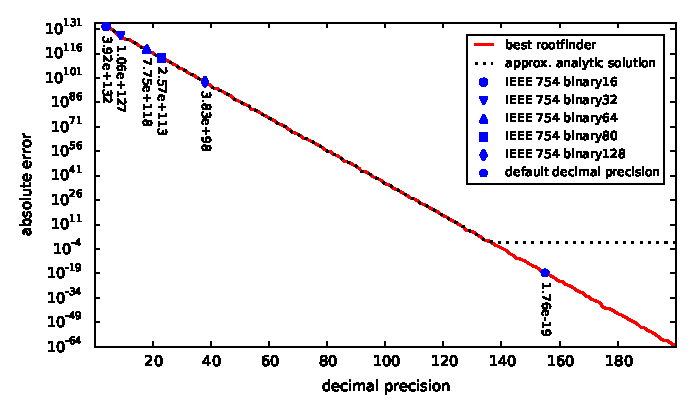
\includegraphics[width=\linewidth]{figures/decimal-precision-error@3-clamped-free-beam.eps}
    \caption{Maximum root-finding errors (across all 100 modes) of clamped-free beam's (LJ=3) characteristic function (EPS image format) \cite{Maric:2017}}
    \label{fig:3-clamped-free-beam-decimal-precision-errors}
\end{figure}

\begin{figure}[H]
    \centering
    \includegraphics[width=\linewidth]{figures/barbero-viscoelastic@local-p1.jpg}
    \caption{Viscoelastic natural frequencies (JPEG image format) \cite{Milasinovic:2018}}
    \label{fig:barbero-viscoelastic-natural-frequencies}
\end{figure}

\begin{figure}[H]
    \centering
    \includegraphics[width=\linewidth]{figures/barbero-viscoelastic@fsm-damage-analysis.pdf}
    \caption{\code{fsm\_damage\_analysis} project example experiment report (PDF image format) \cite{Project:fsm_damage_analysis:CodeRepository}}
    \label{fig:barbero-viscoelastic-damage-analysis}
\end{figure}

  \section*{Supporting information}

% Include only the SI item label in the paragraph heading. Use the \nameref{label} command to cite SI items in the text.
\paragraph*{S1 Fig.}
\label{S1_Fig}
{\bf Bold the title sentence.} Add descriptive text after the title of the item (optional).

\paragraph*{S2 Fig.}
\label{S2_Fig}
{\bf Lorem ipsum.} Maecenas convallis mauris sit amet sem ultrices gravida. Etiam eget sapien nibh. Sed ac ipsum eget enim egestas ullamcorper nec euismod ligula. Curabitur fringilla pulvinar lectus consectetur pellentesque.

\paragraph*{S1 File.}
\label{S1_File}
{\bf Lorem ipsum.}  Maecenas convallis mauris sit amet sem ultrices gravida. Etiam eget sapien nibh. Sed ac ipsum eget enim egestas ullamcorper nec euismod ligula. Curabitur fringilla pulvinar lectus consectetur pellentesque.

\paragraph*{S1 Video.}
\label{S1_Video}
{\bf Lorem ipsum.}  Maecenas convallis mauris sit amet sem ultrices gravida. Etiam eget sapien nibh. Sed ac ipsum eget enim egestas ullamcorper nec euismod ligula. Curabitur fringilla pulvinar lectus consectetur pellentesque.

\paragraph*{S1 Appendix.}
\label{S1_Appendix}
{\bf Lorem ipsum.} Maecenas convallis mauris sit amet sem ultrices gravida. Etiam eget sapien nibh. Sed ac ipsum eget enim egestas ullamcorper nec euismod ligula. Curabitur fringilla pulvinar lectus consectetur pellentesque.

\paragraph*{S1 Table.}
\label{S1_Table}
{\bf Lorem ipsum.} Maecenas convallis mauris sit amet sem ultrices gravida. Etiam eget sapien nibh. Sed ac ipsum eget enim egestas ullamcorper nec euismod ligula. Curabitur fringilla pulvinar lectus consectetur pellentesque.

  \section*{Acknowledgments}
Cras egestas velit mauris, eu mollis turpis pellentesque sit amet. Interdum et malesuada fames ac ante ipsum primis in faucibus. Nam id pretium nisi. Sed ac quam id nisi malesuada congue. Sed interdum aliquet augue, at pellentesque quam rhoncus vitae.


  \nolinenumbers

  % Either type in your references using
  % \begin{thebibliography}{}
  % \bibitem{}
  % Text
  % \end{thebibliography}
  %
  % or
  %
  % Compile your BiBTeX database using our plos2015.bst
  % style file and paste the contents of your .bbl file
  % here. See http://journals.plos.org/plosone/s/latex for
  % step-by-step instructions.
  % \bibliography{references}

  \begin{thebibliography}{10}
    \bibitem{bib1}
    Conant GC, Wolfe KH.
    \newblock {{T}urning a hobby into a job: how duplicated genes find new
      functions}.
    \newblock Nat Rev Genet. 2008 Dec;9(12):938--950.

    \bibitem{bib2}
    Ohno S.
    \newblock Evolution by gene duplication.
    \newblock London: George Alien \& Unwin Ltd. Berlin, Heidelberg and New York:
      Springer-Verlag.; 1970.

    \bibitem{bib3}
    Magwire MM, Bayer F, Webster CL, Cao C, Jiggins FM.
    \newblock {{S}uccessive increases in the resistance of {D}rosophila to viral
      infection through a transposon insertion followed by a {D}uplication}.
    \newblock PLoS Genet. 2011 Oct;7(10):e1002337.

  \end{thebibliography}
\end{document}
